% Created by tikzDevice version 0.12.3.1 on 2023-02-17 13:47:18
% !TEX encoding = UTF-8 Unicode
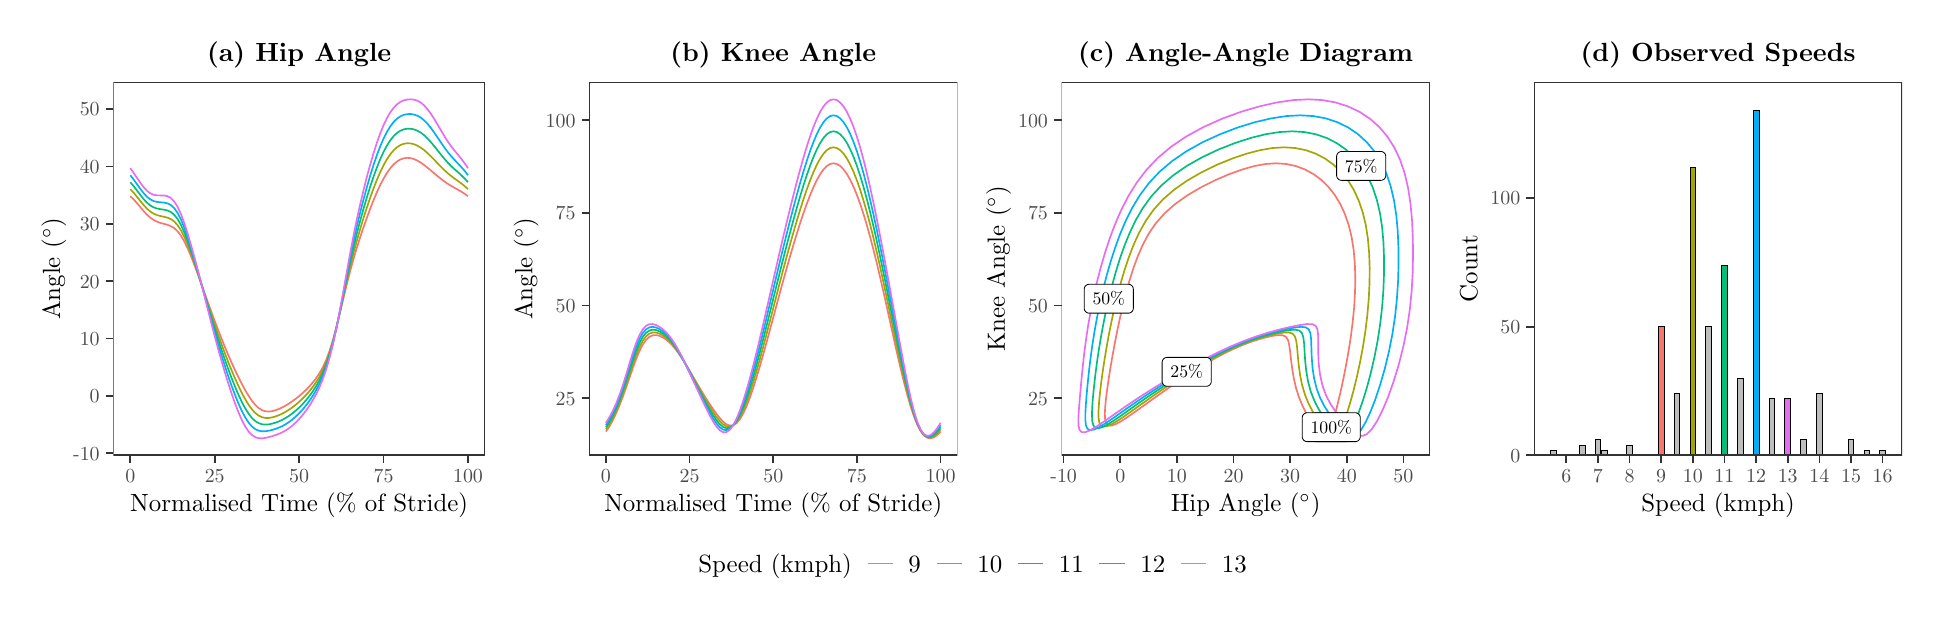
\begin{tikzpicture}[x=1pt,y=1pt]
\definecolor{fillColor}{RGB}{255,255,255}
\path[use as bounding box,fill=fillColor,fill opacity=0.00] (0,0) rectangle (682.86,204.86);
\begin{scope}
\path[clip] (  0.00, 22.44) rectangle (170.72,204.86);
\definecolor{drawColor}{RGB}{255,255,255}
\definecolor{fillColor}{RGB}{255,255,255}

\path[draw=drawColor,line width= 0.6pt,line join=round,line cap=round,fill=fillColor] ( -0.00, 22.44) rectangle (170.72,204.86);
\end{scope}
\begin{scope}
\path[clip] ( 30.98, 50.33) rectangle (165.22,185.10);
\definecolor{fillColor}{RGB}{255,255,255}

\path[fill=fillColor] ( 30.98, 50.33) rectangle (165.22,185.10);
\definecolor{drawColor}{RGB}{248,118,109}

\path[draw=drawColor,line width= 0.6pt,line join=round] ( 37.09,143.96) --
	( 38.31,142.79) --
	( 39.53,141.44) --
	( 40.75,139.97) --
	( 41.97,138.52) --
	( 43.19,137.21) --
	( 44.41,136.13) --
	( 45.63,135.31) --
	( 46.85,134.71) --
	( 48.07,134.28) --
	( 49.29,133.95) --
	( 50.51,133.62) --
	( 51.73,133.16) --
	( 52.95,132.43) --
	( 54.17,131.29) --
	( 55.39,129.69) --
	( 56.61,127.60) --
	( 57.83,125.08) --
	( 59.05,122.20) --
	( 60.27,119.06) --
	( 61.49,115.76) --
	( 62.71,112.37) --
	( 63.93,108.95) --
	( 65.15,105.54) --
	( 66.37,102.17) --
	( 67.59, 98.86) --
	( 68.81, 95.64) --
	( 70.03, 92.52) --
	( 71.25, 89.51) --
	( 72.47, 86.60) --
	( 73.69, 83.82) --
	( 74.91, 81.15) --
	( 76.13, 78.60) --
	( 77.35, 76.19) --
	( 78.58, 73.93) --
	( 79.80, 71.86) --
	( 81.02, 70.04) --
	( 82.24, 68.55) --
	( 83.46, 67.41) --
	( 84.68, 66.65) --
	( 85.90, 66.25) --
	( 87.12, 66.15) --
	( 88.34, 66.29) --
	( 89.56, 66.62) --
	( 90.78, 67.07) --
	( 92.00, 67.64) --
	( 93.22, 68.30) --
	( 94.44, 69.05) --
	( 95.66, 69.87) --
	( 96.88, 70.77) --
	( 98.10, 71.74) --
	( 99.32, 72.79) --
	(100.54, 73.94) --
	(101.76, 75.20) --
	(102.98, 76.60) --
	(104.20, 78.17) --
	(105.42, 79.97) --
	(106.64, 82.12) --
	(107.86, 84.75) --
	(109.08, 88.00) --
	(110.30, 91.93) --
	(111.52, 96.46) --
	(112.74,101.42) --
	(113.96,106.55) --
	(115.18,111.60) --
	(116.40,116.41) --
	(117.62,120.87) --
	(118.84,125.00) --
	(120.07,128.87) --
	(121.29,132.52) --
	(122.51,136.01) --
	(123.73,139.33) --
	(124.95,142.46) --
	(126.17,145.36) --
	(127.39,147.99) --
	(128.61,150.34) --
	(129.83,152.38) --
	(131.05,154.09) --
	(132.27,155.47) --
	(133.49,156.52) --
	(134.71,157.25) --
	(135.93,157.67) --
	(137.15,157.82) --
	(138.37,157.72) --
	(139.59,157.38) --
	(140.81,156.83) --
	(142.03,156.10) --
	(143.25,155.24) --
	(144.47,154.27) --
	(145.69,153.26) --
	(146.91,152.23) --
	(148.13,151.20) --
	(149.35,150.22) --
	(150.57,149.29) --
	(151.79,148.45) --
	(153.01,147.69) --
	(154.23,146.99) --
	(155.45,146.32) --
	(156.67,145.63) --
	(157.89,144.85) --
	(159.11,143.95);
\definecolor{drawColor}{RGB}{163,165,0}

\path[draw=drawColor,line width= 0.6pt,line join=round] ( 37.09,146.49) --
	( 38.31,145.18) --
	( 39.53,143.71) --
	( 40.75,142.17) --
	( 41.97,140.68) --
	( 43.19,139.37) --
	( 44.41,138.34) --
	( 45.63,137.60) --
	( 46.85,137.10) --
	( 48.07,136.77) --
	( 49.29,136.51) --
	( 50.51,136.21) --
	( 51.73,135.70) --
	( 52.95,134.84) --
	( 54.17,133.50) --
	( 55.39,131.64) --
	( 56.61,129.25) --
	( 57.83,126.41) --
	( 59.05,123.20) --
	( 60.27,119.75) --
	( 61.49,116.13) --
	( 62.71,112.40) --
	( 63.93,108.64) --
	( 65.15,104.87) --
	( 66.37,101.14) --
	( 67.59, 97.49) --
	( 68.81, 93.94) --
	( 70.03, 90.52) --
	( 71.25, 87.22) --
	( 72.47, 84.05) --
	( 73.69, 81.03) --
	( 74.91, 78.16) --
	( 76.13, 75.45) --
	( 77.35, 72.93) --
	( 78.58, 70.65) --
	( 79.80, 68.63) --
	( 81.02, 66.95) --
	( 82.24, 65.63) --
	( 83.46, 64.68) --
	( 84.68, 64.10) --
	( 85.90, 63.84) --
	( 87.12, 63.84) --
	( 88.34, 64.03) --
	( 89.56, 64.37) --
	( 90.78, 64.83) --
	( 92.00, 65.39) --
	( 93.22, 66.06) --
	( 94.44, 66.82) --
	( 95.66, 67.67) --
	( 96.88, 68.62) --
	( 98.10, 69.67) --
	( 99.32, 70.81) --
	(100.54, 72.06) --
	(101.76, 73.44) --
	(102.98, 74.98) --
	(104.20, 76.71) --
	(105.42, 78.70) --
	(106.64, 81.06) --
	(107.86, 83.91) --
	(109.08, 87.39) --
	(110.30, 91.55) --
	(111.52, 96.35) --
	(112.74,101.63) --
	(113.96,107.15) --
	(115.18,112.66) --
	(116.40,117.96) --
	(117.62,122.92) --
	(118.84,127.53) --
	(120.07,131.83) --
	(121.29,135.86) --
	(122.51,139.69) --
	(123.73,143.31) --
	(124.95,146.70) --
	(126.17,149.82) --
	(127.39,152.66) --
	(128.61,155.17) --
	(129.83,157.33) --
	(131.05,159.14) --
	(132.27,160.58) --
	(133.49,161.68) --
	(134.71,162.45) --
	(135.93,162.90) --
	(137.15,163.09) --
	(138.37,163.03) --
	(139.59,162.74) --
	(140.81,162.24) --
	(142.03,161.52) --
	(143.25,160.62) --
	(144.47,159.56) --
	(145.69,158.38) --
	(146.91,157.13) --
	(148.13,155.85) --
	(149.35,154.59) --
	(150.57,153.39) --
	(151.79,152.27) --
	(153.01,151.27) --
	(154.23,150.36) --
	(155.45,149.49) --
	(156.67,148.59) --
	(157.89,147.61) --
	(159.11,146.49);
\definecolor{drawColor}{RGB}{0,191,125}

\path[draw=drawColor,line width= 0.6pt,line join=round] ( 37.09,149.02) --
	( 38.31,147.57) --
	( 39.53,145.99) --
	( 40.75,144.37) --
	( 41.97,142.83) --
	( 43.19,141.53) --
	( 44.41,140.54) --
	( 45.63,139.88) --
	( 46.85,139.49) --
	( 48.07,139.26) --
	( 49.29,139.08) --
	( 50.51,138.79) --
	( 51.73,138.24) --
	( 52.95,137.25) --
	( 54.17,135.72) --
	( 55.39,133.59) --
	( 56.61,130.90) --
	( 57.83,127.73) --
	( 59.05,124.21) --
	( 60.27,120.43) --
	( 61.49,116.49) --
	( 62.71,112.44) --
	( 63.93,108.32) --
	( 65.15,104.20) --
	( 66.37,100.12) --
	( 67.59, 96.12) --
	( 68.81, 92.24) --
	( 70.03, 88.51) --
	( 71.25, 84.92) --
	( 72.47, 81.50) --
	( 73.69, 78.24) --
	( 74.91, 75.16) --
	( 76.13, 72.29) --
	( 77.35, 69.67) --
	( 78.58, 67.37) --
	( 79.80, 65.41) --
	( 81.02, 63.85) --
	( 82.24, 62.71) --
	( 83.46, 61.96) --
	( 84.68, 61.55) --
	( 85.90, 61.43) --
	( 87.12, 61.52) --
	( 88.34, 61.77) --
	( 89.56, 62.13) --
	( 90.78, 62.58) --
	( 92.00, 63.14) --
	( 93.22, 63.81) --
	( 94.44, 64.59) --
	( 95.66, 65.48) --
	( 96.88, 66.48) --
	( 98.10, 67.59) --
	( 99.32, 68.82) --
	(100.54, 70.18) --
	(101.76, 71.68) --
	(102.98, 73.36) --
	(104.20, 75.26) --
	(105.42, 77.43) --
	(106.64, 79.99) --
	(107.86, 83.07) --
	(109.08, 86.77) --
	(110.30, 91.17) --
	(111.52, 96.24) --
	(112.74,101.85) --
	(113.96,107.75) --
	(115.18,113.72) --
	(116.40,119.51) --
	(117.62,124.98) --
	(118.84,130.06) --
	(120.07,134.78) --
	(121.29,139.20) --
	(122.51,143.36) --
	(123.73,147.28) --
	(124.95,150.93) --
	(126.17,154.29) --
	(127.39,157.32) --
	(128.61,159.99) --
	(129.83,162.28) --
	(131.05,164.18) --
	(132.27,165.70) --
	(133.49,166.84) --
	(134.71,167.64) --
	(135.93,168.13) --
	(137.15,168.36) --
	(138.37,168.34) --
	(139.59,168.11) --
	(140.81,167.65) --
	(142.03,166.95) --
	(143.25,166.01) --
	(144.47,164.85) --
	(145.69,163.51) --
	(146.91,162.04) --
	(148.13,160.51) --
	(149.35,158.96) --
	(150.57,157.48) --
	(151.79,156.10) --
	(153.01,154.85) --
	(154.23,153.73) --
	(155.45,152.65) --
	(156.67,151.56) --
	(157.89,150.36) --
	(159.11,149.02);
\definecolor{drawColor}{RGB}{0,176,246}

\path[draw=drawColor,line width= 0.6pt,line join=round] ( 37.09,151.55) --
	( 38.31,149.96) --
	( 39.53,148.27) --
	( 40.75,146.56) --
	( 41.97,144.99) --
	( 43.19,143.69) --
	( 44.41,142.75) --
	( 45.63,142.16) --
	( 46.85,141.87) --
	( 48.07,141.75) --
	( 49.29,141.65) --
	( 50.51,141.38) --
	( 51.73,140.77) --
	( 52.95,139.66) --
	( 54.17,137.93) --
	( 55.39,135.54) --
	( 56.61,132.55) --
	( 57.83,129.06) --
	( 59.05,125.21) --
	( 60.27,121.12) --
	( 61.49,116.85) --
	( 62.71,112.47) --
	( 63.93,108.01) --
	( 65.15,103.53) --
	( 66.37, 99.09) --
	( 67.59, 94.75) --
	( 68.81, 90.54) --
	( 70.03, 86.50) --
	( 71.25, 82.63) --
	( 72.47, 78.94) --
	( 73.69, 75.44) --
	( 74.91, 72.16) --
	( 76.13, 69.13) --
	( 77.35, 66.42) --
	( 78.58, 64.09) --
	( 79.80, 62.19) --
	( 81.02, 60.76) --
	( 82.24, 59.79) --
	( 83.46, 59.23) --
	( 84.68, 59.01) --
	( 85.90, 59.03) --
	( 87.12, 59.21) --
	( 88.34, 59.50) --
	( 89.56, 59.88) --
	( 90.78, 60.34) --
	( 92.00, 60.89) --
	( 93.22, 61.56) --
	( 94.44, 62.36) --
	( 95.66, 63.28) --
	( 96.88, 64.33) --
	( 98.10, 65.52) --
	( 99.32, 66.84) --
	(100.54, 68.30) --
	(101.76, 69.93) --
	(102.98, 71.74) --
	(104.20, 73.80) --
	(105.42, 76.16) --
	(106.64, 78.93) --
	(107.86, 82.22) --
	(109.08, 86.15) --
	(110.30, 90.79) --
	(111.52, 96.13) --
	(112.74,102.06) --
	(113.96,108.36) --
	(115.18,114.78) --
	(116.40,121.07) --
	(117.62,127.03) --
	(118.84,132.59) --
	(120.07,137.74) --
	(121.29,142.54) --
	(122.51,147.04) --
	(123.73,151.25) --
	(124.95,155.17) --
	(126.17,158.76) --
	(127.39,161.98) --
	(128.61,164.81) --
	(129.83,167.23) --
	(131.05,169.23) --
	(132.27,170.81) --
	(133.49,172.00) --
	(134.71,172.84) --
	(135.93,173.36) --
	(137.15,173.62) --
	(138.37,173.66) --
	(139.59,173.47) --
	(140.81,173.06) --
	(142.03,172.37) --
	(143.25,171.39) --
	(144.47,170.14) --
	(145.69,168.63) --
	(146.91,166.95) --
	(148.13,165.16) --
	(149.35,163.34) --
	(150.57,161.57) --
	(151.79,159.92) --
	(153.01,158.44) --
	(154.23,157.09) --
	(155.45,155.82) --
	(156.67,154.52) --
	(157.89,153.12) --
	(159.11,151.56);
\definecolor{drawColor}{RGB}{231,107,243}

\path[draw=drawColor,line width= 0.6pt,line join=round] ( 37.09,154.08) --
	( 38.31,152.36) --
	( 39.53,150.54) --
	( 40.75,148.76) --
	( 41.97,147.15) --
	( 43.19,145.85) --
	( 44.41,144.95) --
	( 45.63,144.45) --
	( 46.85,144.26) --
	( 48.07,144.24) --
	( 49.29,144.21) --
	( 50.51,143.97) --
	( 51.73,143.31) --
	( 52.95,142.07) --
	( 54.17,140.14) --
	( 55.39,137.49) --
	( 56.61,134.19) --
	( 57.83,130.38) --
	( 59.05,126.21) --
	( 60.27,121.80) --
	( 61.49,117.21) --
	( 62.71,112.50) --
	( 63.93,107.70) --
	( 65.15,102.86) --
	( 66.37, 98.06) --
	( 67.59, 93.38) --
	( 68.81, 88.84) --
	( 70.03, 84.49) --
	( 71.25, 80.34) --
	( 72.47, 76.39) --
	( 73.69, 72.65) --
	( 74.91, 69.16) --
	( 76.13, 65.97) --
	( 77.35, 63.16) --
	( 78.58, 60.81) --
	( 79.80, 58.97) --
	( 81.02, 57.67) --
	( 82.24, 56.87) --
	( 83.46, 56.50) --
	( 84.68, 56.46) --
	( 85.90, 56.62) --
	( 87.12, 56.90) --
	( 88.34, 57.24) --
	( 89.56, 57.63) --
	( 90.78, 58.09) --
	( 92.00, 58.64) --
	( 93.22, 59.32) --
	( 94.44, 60.12) --
	( 95.66, 61.08) --
	( 96.88, 62.19) --
	( 98.10, 63.45) --
	( 99.32, 64.86) --
	(100.54, 66.43) --
	(101.76, 68.17) --
	(102.98, 70.13) --
	(104.20, 72.34) --
	(105.42, 74.89) --
	(106.64, 77.87) --
	(107.86, 81.38) --
	(109.08, 85.54) --
	(110.30, 90.41) --
	(111.52, 96.02) --
	(112.74,102.27) --
	(113.96,108.96) --
	(115.18,115.84) --
	(116.40,122.62) --
	(117.62,129.09) --
	(118.84,135.12) --
	(120.07,140.70) --
	(121.29,145.88) --
	(122.51,150.72) --
	(123.73,155.22) --
	(124.95,159.40) --
	(126.17,163.22) --
	(127.39,166.65) --
	(128.61,169.64) --
	(129.83,172.18) --
	(131.05,174.28) --
	(132.27,175.93) --
	(133.49,177.17) --
	(134.71,178.04) --
	(135.93,178.59) --
	(137.15,178.89) --
	(138.37,178.97) --
	(139.59,178.84) --
	(140.81,178.47) --
	(142.03,177.79) --
	(143.25,176.78) --
	(144.47,175.42) --
	(145.69,173.76) --
	(146.91,171.86) --
	(148.13,169.81) --
	(149.35,167.71) --
	(150.57,165.66) --
	(151.79,163.75) --
	(153.01,162.02) --
	(154.23,160.46) --
	(155.45,158.99) --
	(156.67,157.49) --
	(157.89,155.87) --
	(159.11,154.09);
\definecolor{drawColor}{gray}{0.20}

\path[draw=drawColor,line width= 0.6pt,line join=round,line cap=round] ( 30.98, 50.33) rectangle (165.22,185.10);
\end{scope}
\begin{scope}
\path[clip] (  0.00,  0.00) rectangle (682.86,204.86);
\definecolor{drawColor}{gray}{0.30}

\node[text=drawColor,anchor=base east,inner sep=0pt, outer sep=0pt, scale=  0.72] at ( 26.03, 48.60) {-10};

\node[text=drawColor,anchor=base east,inner sep=0pt, outer sep=0pt, scale=  0.72] at ( 26.03, 69.33) {0};

\node[text=drawColor,anchor=base east,inner sep=0pt, outer sep=0pt, scale=  0.72] at ( 26.03, 90.06) {10};

\node[text=drawColor,anchor=base east,inner sep=0pt, outer sep=0pt, scale=  0.72] at ( 26.03,110.79) {20};

\node[text=drawColor,anchor=base east,inner sep=0pt, outer sep=0pt, scale=  0.72] at ( 26.03,131.52) {30};

\node[text=drawColor,anchor=base east,inner sep=0pt, outer sep=0pt, scale=  0.72] at ( 26.03,152.25) {40};

\node[text=drawColor,anchor=base east,inner sep=0pt, outer sep=0pt, scale=  0.72] at ( 26.03,172.98) {50};
\end{scope}
\begin{scope}
\path[clip] (  0.00,  0.00) rectangle (682.86,204.86);
\definecolor{drawColor}{gray}{0.20}

\path[draw=drawColor,line width= 0.6pt,line join=round] ( 28.23, 51.08) --
	( 30.98, 51.08);

\path[draw=drawColor,line width= 0.6pt,line join=round] ( 28.23, 71.81) --
	( 30.98, 71.81);

\path[draw=drawColor,line width= 0.6pt,line join=round] ( 28.23, 92.54) --
	( 30.98, 92.54);

\path[draw=drawColor,line width= 0.6pt,line join=round] ( 28.23,113.27) --
	( 30.98,113.27);

\path[draw=drawColor,line width= 0.6pt,line join=round] ( 28.23,134.00) --
	( 30.98,134.00);

\path[draw=drawColor,line width= 0.6pt,line join=round] ( 28.23,154.73) --
	( 30.98,154.73);

\path[draw=drawColor,line width= 0.6pt,line join=round] ( 28.23,175.46) --
	( 30.98,175.46);
\end{scope}
\begin{scope}
\path[clip] (  0.00,  0.00) rectangle (682.86,204.86);
\definecolor{drawColor}{gray}{0.20}

\path[draw=drawColor,line width= 0.6pt,line join=round] ( 37.09, 47.58) --
	( 37.09, 50.33);

\path[draw=drawColor,line width= 0.6pt,line join=round] ( 67.59, 47.58) --
	( 67.59, 50.33);

\path[draw=drawColor,line width= 0.6pt,line join=round] ( 98.10, 47.58) --
	( 98.10, 50.33);

\path[draw=drawColor,line width= 0.6pt,line join=round] (128.61, 47.58) --
	(128.61, 50.33);

\path[draw=drawColor,line width= 0.6pt,line join=round] (159.11, 47.58) --
	(159.11, 50.33);
\end{scope}
\begin{scope}
\path[clip] (  0.00,  0.00) rectangle (682.86,204.86);
\definecolor{drawColor}{gray}{0.30}

\node[text=drawColor,anchor=base,inner sep=0pt, outer sep=0pt, scale=  0.72] at ( 37.09, 40.42) {0};

\node[text=drawColor,anchor=base,inner sep=0pt, outer sep=0pt, scale=  0.72] at ( 67.59, 40.42) {25};

\node[text=drawColor,anchor=base,inner sep=0pt, outer sep=0pt, scale=  0.72] at ( 98.10, 40.42) {50};

\node[text=drawColor,anchor=base,inner sep=0pt, outer sep=0pt, scale=  0.72] at (128.61, 40.42) {75};

\node[text=drawColor,anchor=base,inner sep=0pt, outer sep=0pt, scale=  0.72] at (159.11, 40.42) {100};
\end{scope}
\begin{scope}
\path[clip] (  0.00,  0.00) rectangle (682.86,204.86);
\definecolor{drawColor}{RGB}{0,0,0}

\node[text=drawColor,anchor=base,inner sep=0pt, outer sep=0pt, scale=  0.90] at ( 98.10, 29.93) {Normalised Time ($\%$ of Stride)};
\end{scope}
\begin{scope}
\path[clip] (  0.00,  0.00) rectangle (682.86,204.86);
\definecolor{drawColor}{RGB}{0,0,0}

\node[text=drawColor,rotate= 90.00,anchor=base,inner sep=0pt, outer sep=0pt, scale=  0.90] at ( 11.70,117.71) {Angle ($^{\circ}$)};
\end{scope}
\begin{scope}
\path[clip] (  0.00,  0.00) rectangle (682.86,204.86);
\definecolor{drawColor}{RGB}{0,0,0}

\node[text=drawColor,anchor=base,inner sep=0pt, outer sep=0pt, scale=  0.95] at ( 98.10,192.80) {\bfseries (a) Hip Angle};
\end{scope}
\begin{scope}
\path[clip] (170.72, 22.44) rectangle (341.43,204.86);
\definecolor{drawColor}{RGB}{255,255,255}
\definecolor{fillColor}{RGB}{255,255,255}

\path[draw=drawColor,line width= 0.6pt,line join=round,line cap=round,fill=fillColor] (170.72, 22.44) rectangle (341.43,204.86);
\end{scope}
\begin{scope}
\path[clip] (202.90, 50.33) rectangle (335.93,185.10);
\definecolor{fillColor}{RGB}{255,255,255}

\path[fill=fillColor] (202.90, 50.33) rectangle (335.93,185.10);
\definecolor{drawColor}{RGB}{248,118,109}

\path[draw=drawColor,line width= 0.6pt,line join=round] (208.95, 58.93) --
	(210.16, 60.69) --
	(211.37, 62.85) --
	(212.57, 65.37) --
	(213.78, 68.21) --
	(214.99, 71.33) --
	(216.20, 74.68) --
	(217.41, 78.19) --
	(218.62, 81.71) --
	(219.83, 85.05) --
	(221.04, 87.98) --
	(222.25, 90.35) --
	(223.46, 92.08) --
	(224.67, 93.17) --
	(225.88, 93.70) --
	(227.09, 93.78) --
	(228.30, 93.51) --
	(229.51, 92.96) --
	(230.72, 92.16) --
	(231.92, 91.13) --
	(233.13, 89.86) --
	(234.34, 88.38) --
	(235.55, 86.70) --
	(236.76, 84.87) --
	(237.97, 82.92) --
	(239.18, 80.89) --
	(240.39, 78.82) --
	(241.60, 76.75) --
	(242.81, 74.69) --
	(244.02, 72.68) --
	(245.23, 70.73) --
	(246.44, 68.84) --
	(247.65, 67.04) --
	(248.86, 65.35) --
	(250.07, 63.81) --
	(251.28, 62.51) --
	(252.48, 61.55) --
	(253.69, 61.07) --
	(254.90, 61.16) --
	(256.11, 61.91) --
	(257.32, 63.33) --
	(258.53, 65.39) --
	(259.74, 68.03) --
	(260.95, 71.15) --
	(262.16, 74.67) --
	(263.37, 78.50) --
	(264.58, 82.58) --
	(265.79, 86.83) --
	(267.00, 91.21) --
	(268.21, 95.67) --
	(269.42,100.18) --
	(270.63,104.68) --
	(271.83,109.15) --
	(273.04,113.57) --
	(274.25,117.90) --
	(275.46,122.15) --
	(276.67,126.28) --
	(277.88,130.28) --
	(279.09,134.11) --
	(280.30,137.75) --
	(281.51,141.17) --
	(282.72,144.33) --
	(283.93,147.21) --
	(285.14,149.74) --
	(286.35,151.89) --
	(287.56,153.61) --
	(288.77,154.85) --
	(289.98,155.60) --
	(291.18,155.85) --
	(292.39,155.60) --
	(293.60,154.87) --
	(294.81,153.66) --
	(296.02,151.99) --
	(297.23,149.87) --
	(298.44,147.33) --
	(299.65,144.38) --
	(300.86,141.06) --
	(302.07,137.37) --
	(303.28,133.33) --
	(304.49,128.97) --
	(305.70,124.32) --
	(306.91,119.40) --
	(308.12,114.27) --
	(309.33,108.97) --
	(310.54,103.54) --
	(311.74, 98.06) --
	(312.95, 92.60) --
	(314.16, 87.22) --
	(315.37, 82.00) --
	(316.58, 77.03) --
	(317.79, 72.40) --
	(319.00, 68.20) --
	(320.21, 64.53) --
	(321.42, 61.49) --
	(322.63, 59.15) --
	(323.84, 57.55) --
	(325.05, 56.68) --
	(326.26, 56.46) --
	(327.47, 56.82) --
	(328.68, 57.67) --
	(329.89, 58.94);
\definecolor{drawColor}{RGB}{163,165,0}

\path[draw=drawColor,line width= 0.6pt,line join=round] (208.95, 59.71) --
	(210.16, 61.51) --
	(211.37, 63.70) --
	(212.57, 66.25) --
	(213.78, 69.14) --
	(214.99, 72.35) --
	(216.20, 75.83) --
	(217.41, 79.47) --
	(218.62, 83.10) --
	(219.83, 86.49) --
	(221.04, 89.42) --
	(222.25, 91.72) --
	(223.46, 93.34) --
	(224.67, 94.31) --
	(225.88, 94.71) --
	(227.09, 94.68) --
	(228.30, 94.32) --
	(229.51, 93.68) --
	(230.72, 92.81) --
	(231.92, 91.69) --
	(233.13, 90.33) --
	(234.34, 88.73) --
	(235.55, 86.93) --
	(236.76, 84.95) --
	(237.97, 82.86) --
	(239.18, 80.69) --
	(240.39, 78.49) --
	(241.60, 76.28) --
	(242.81, 74.10) --
	(244.02, 71.95) --
	(245.23, 69.85) --
	(246.44, 67.84) --
	(247.65, 65.94) --
	(248.86, 64.20) --
	(250.07, 62.71) --
	(251.28, 61.55) --
	(252.48, 60.84) --
	(253.69, 60.69) --
	(254.90, 61.16) --
	(256.11, 62.30) --
	(257.32, 64.10) --
	(258.53, 66.52) --
	(259.74, 69.48) --
	(260.95, 72.89) --
	(262.16, 76.68) --
	(263.37, 80.76) --
	(264.58, 85.07) --
	(265.79, 89.56) --
	(267.00, 94.17) --
	(268.21, 98.84) --
	(269.42,103.55) --
	(270.63,108.25) --
	(271.83,112.91) --
	(273.04,117.51) --
	(274.25,122.03) --
	(275.46,126.46) --
	(276.67,130.77) --
	(277.88,134.94) --
	(279.09,138.95) --
	(280.30,142.76) --
	(281.51,146.34) --
	(282.72,149.64) --
	(283.93,152.64) --
	(285.14,155.29) --
	(286.35,157.52) --
	(287.56,159.30) --
	(288.77,160.59) --
	(289.98,161.37) --
	(291.18,161.63) --
	(292.39,161.37) --
	(293.60,160.60) --
	(294.81,159.34) --
	(296.02,157.60) --
	(297.23,155.38) --
	(298.44,152.73) --
	(299.65,149.64) --
	(300.86,146.15) --
	(302.07,142.27) --
	(303.28,138.03) --
	(304.49,133.45) --
	(305.70,128.55) --
	(306.91,123.38) --
	(308.12,117.99) --
	(309.33,112.42) --
	(310.54,106.73) --
	(311.74,100.97) --
	(312.95, 95.21) --
	(314.16, 89.50) --
	(315.37, 83.93) --
	(316.58, 78.57) --
	(317.79, 73.55) --
	(319.00, 68.98) --
	(320.21, 65.00) --
	(321.42, 61.74) --
	(322.63, 59.28) --
	(323.84, 57.66) --
	(325.05, 56.84) --
	(326.26, 56.75) --
	(327.47, 57.27) --
	(328.68, 58.29) --
	(329.89, 59.72);
\definecolor{drawColor}{RGB}{0,191,125}

\path[draw=drawColor,line width= 0.6pt,line join=round] (208.95, 60.48) --
	(210.16, 62.34) --
	(211.37, 64.55) --
	(212.57, 67.12) --
	(213.78, 70.06) --
	(214.99, 73.37) --
	(216.20, 76.98) --
	(217.41, 80.76) --
	(218.62, 84.49) --
	(219.83, 87.94) --
	(221.04, 90.85) --
	(222.25, 93.09) --
	(223.46, 94.60) --
	(224.67, 95.44) --
	(225.88, 95.73) --
	(227.09, 95.59) --
	(228.30, 95.13) --
	(229.51, 94.41) --
	(230.72, 93.45) --
	(231.92, 92.25) --
	(233.13, 90.79) --
	(234.34, 89.08) --
	(235.55, 87.15) --
	(236.76, 85.03) --
	(237.97, 82.80) --
	(239.18, 80.49) --
	(240.39, 78.16) --
	(241.60, 75.82) --
	(242.81, 73.50) --
	(244.02, 71.22) --
	(245.23, 68.98) --
	(246.44, 66.83) --
	(247.65, 64.83) --
	(248.86, 63.05) --
	(250.07, 61.60) --
	(251.28, 60.59) --
	(252.48, 60.13) --
	(253.69, 60.30) --
	(254.90, 61.15) --
	(256.11, 62.69) --
	(257.32, 64.88) --
	(258.53, 67.65) --
	(259.74, 70.93) --
	(260.95, 74.63) --
	(262.16, 78.68) --
	(263.37, 83.01) --
	(264.58, 87.57) --
	(265.79, 92.29) --
	(267.00, 97.12) --
	(268.21,102.01) --
	(269.42,106.92) --
	(270.63,111.81) --
	(271.83,116.66) --
	(273.04,121.45) --
	(274.25,126.15) --
	(275.46,130.76) --
	(276.67,135.25) --
	(277.88,139.60) --
	(279.09,143.79) --
	(280.30,147.77) --
	(281.51,151.50) --
	(282.72,154.96) --
	(283.93,158.08) --
	(285.14,160.83) --
	(286.35,163.15) --
	(287.56,165.00) --
	(288.77,166.34) --
	(289.98,167.14) --
	(291.18,167.41) --
	(292.39,167.14) --
	(293.60,166.34) --
	(294.81,165.03) --
	(296.02,163.21) --
	(297.23,160.90) --
	(298.44,158.13) --
	(299.65,154.90) --
	(300.86,151.24) --
	(302.07,147.18) --
	(303.28,142.73) --
	(304.49,137.92) --
	(305.70,132.78) --
	(306.91,127.36) --
	(308.12,121.70) --
	(309.33,115.87) --
	(310.54,109.91) --
	(311.74,103.88) --
	(312.95, 97.82) --
	(314.16, 91.78) --
	(315.37, 85.85) --
	(316.58, 80.12) --
	(317.79, 74.70) --
	(319.00, 69.77) --
	(320.21, 65.48) --
	(321.42, 61.99) --
	(322.63, 59.40) --
	(323.84, 57.76) --
	(325.05, 57.01) --
	(326.26, 57.04) --
	(327.47, 57.72) --
	(328.68, 58.91) --
	(329.89, 60.49);
\definecolor{drawColor}{RGB}{0,176,246}

\path[draw=drawColor,line width= 0.6pt,line join=round] (208.95, 61.26) --
	(210.16, 63.17) --
	(211.37, 65.40) --
	(212.57, 68.00) --
	(213.78, 70.99) --
	(214.99, 74.39) --
	(216.20, 78.13) --
	(217.41, 82.04) --
	(218.62, 85.88) --
	(219.83, 89.38) --
	(221.04, 92.29) --
	(222.25, 94.46) --
	(223.46, 95.86) --
	(224.67, 96.58) --
	(225.88, 96.75) --
	(227.09, 96.50) --
	(228.30, 95.94) --
	(229.51, 95.14) --
	(230.72, 94.10) --
	(231.92, 92.81) --
	(233.13, 91.25) --
	(234.34, 89.43) --
	(235.55, 87.37) --
	(236.76, 85.12) --
	(237.97, 82.74) --
	(239.18, 80.30) --
	(240.39, 77.83) --
	(241.60, 75.36) --
	(242.81, 72.91) --
	(244.02, 70.48) --
	(245.23, 68.11) --
	(246.44, 65.83) --
	(247.65, 63.73) --
	(248.86, 61.91) --
	(250.07, 60.50) --
	(251.28, 59.63) --
	(252.48, 59.42) --
	(253.69, 59.92) --
	(254.90, 61.15) --
	(256.11, 63.08) --
	(257.32, 65.65) --
	(258.53, 68.78) --
	(259.74, 72.38) --
	(260.95, 76.37) --
	(262.16, 80.68) --
	(263.37, 85.27) --
	(264.58, 90.07) --
	(265.79, 95.02) --
	(267.00,100.07) --
	(268.21,105.18) --
	(269.42,110.29) --
	(270.63,115.38) --
	(271.83,120.42) --
	(273.04,125.39) --
	(274.25,130.28) --
	(275.46,135.06) --
	(276.67,139.73) --
	(277.88,144.27) --
	(279.09,148.63) --
	(280.30,152.78) --
	(281.51,156.67) --
	(282.72,160.27) --
	(283.93,163.52) --
	(285.14,166.37) --
	(286.35,168.78) --
	(287.56,170.70) --
	(288.77,172.08) --
	(289.98,172.92) --
	(291.18,173.19) --
	(292.39,172.91) --
	(293.60,172.08) --
	(294.81,170.71) --
	(296.02,168.82) --
	(297.23,166.42) --
	(298.44,163.53) --
	(299.65,160.16) --
	(300.86,156.34) --
	(302.07,152.09) --
	(303.28,147.43) --
	(304.49,142.39) --
	(305.70,137.01) --
	(306.91,131.33) --
	(308.12,125.42) --
	(309.33,119.32) --
	(310.54,113.10) --
	(311.74,106.79) --
	(312.95,100.43) --
	(314.16, 94.07) --
	(315.37, 87.78) --
	(316.58, 81.66) --
	(317.79, 75.85) --
	(319.00, 70.55) --
	(320.21, 65.96) --
	(321.42, 62.24) --
	(322.63, 59.53) --
	(323.84, 57.86) --
	(325.05, 57.17) --
	(326.26, 57.34) --
	(327.47, 58.18) --
	(328.68, 59.53) --
	(329.89, 61.27);
\definecolor{drawColor}{RGB}{231,107,243}

\path[draw=drawColor,line width= 0.6pt,line join=round] (208.95, 62.04) --
	(210.16, 64.00) --
	(211.37, 66.26) --
	(212.57, 68.87) --
	(213.78, 71.92) --
	(214.99, 75.41) --
	(216.20, 79.28) --
	(217.41, 83.32) --
	(218.62, 87.28) --
	(219.83, 90.83) --
	(221.04, 93.72) --
	(222.25, 95.82) --
	(223.46, 97.12) --
	(224.67, 97.72) --
	(225.88, 97.76) --
	(227.09, 97.40) --
	(228.30, 96.75) --
	(229.51, 95.86) --
	(230.72, 94.74) --
	(231.92, 93.37) --
	(233.13, 91.72) --
	(234.34, 89.78) --
	(235.55, 87.59) --
	(236.76, 85.20) --
	(237.97, 82.68) --
	(239.18, 80.10) --
	(240.39, 77.50) --
	(241.60, 74.90) --
	(242.81, 72.32) --
	(244.02, 69.75) --
	(245.23, 67.24) --
	(246.44, 64.82) --
	(247.65, 62.62) --
	(248.86, 60.76) --
	(250.07, 59.40) --
	(251.28, 58.68) --
	(252.48, 58.71) --
	(253.69, 59.53) --
	(254.90, 61.14) --
	(256.11, 63.47) --
	(257.32, 66.43) --
	(258.53, 69.91) --
	(259.74, 73.83) --
	(260.95, 78.10) --
	(262.16, 82.69) --
	(263.37, 87.52) --
	(264.58, 92.56) --
	(265.79, 97.75) --
	(267.00,103.03) --
	(268.21,108.35) --
	(269.42,113.67) --
	(270.63,118.95) --
	(271.83,124.18) --
	(273.04,129.33) --
	(274.25,134.40) --
	(275.46,139.37) --
	(276.67,144.22) --
	(277.88,148.93) --
	(279.09,153.47) --
	(280.30,157.79) --
	(281.51,161.84) --
	(282.72,165.58) --
	(283.93,168.95) --
	(285.14,171.91) --
	(286.35,174.41) --
	(287.56,176.39) --
	(288.77,177.83) --
	(289.98,178.69) --
	(291.18,178.97) --
	(292.39,178.68) --
	(293.60,177.81) --
	(294.81,176.39) --
	(296.02,174.43) --
	(297.23,171.94) --
	(298.44,168.93) --
	(299.65,165.41) --
	(300.86,161.43) --
	(302.07,156.99) --
	(303.28,152.13) --
	(304.49,146.86) --
	(305.70,141.24) --
	(306.91,135.31) --
	(308.12,129.13) --
	(309.33,122.77) --
	(310.54,116.28) --
	(311.74,109.70) --
	(312.95,103.04) --
	(314.16, 96.35) --
	(315.37, 89.70) --
	(316.58, 83.20) --
	(317.79, 77.00) --
	(319.00, 71.34) --
	(320.21, 66.44) --
	(321.42, 62.49) --
	(322.63, 59.65) --
	(323.84, 57.96) --
	(325.05, 57.34) --
	(326.26, 57.63) --
	(327.47, 58.63) --
	(328.68, 60.15) --
	(329.89, 62.05);
\definecolor{drawColor}{gray}{0.20}

\path[draw=drawColor,line width= 0.6pt,line join=round,line cap=round] (202.90, 50.33) rectangle (335.93,185.10);
\end{scope}
\begin{scope}
\path[clip] (  0.00,  0.00) rectangle (682.86,204.86);
\definecolor{drawColor}{gray}{0.30}

\node[text=drawColor,anchor=base east,inner sep=0pt, outer sep=0pt, scale=  0.72] at (197.95, 68.48) {25};

\node[text=drawColor,anchor=base east,inner sep=0pt, outer sep=0pt, scale=  0.72] at (197.95,101.97) {50};

\node[text=drawColor,anchor=base east,inner sep=0pt, outer sep=0pt, scale=  0.72] at (197.95,135.46) {75};

\node[text=drawColor,anchor=base east,inner sep=0pt, outer sep=0pt, scale=  0.72] at (197.95,168.94) {100};
\end{scope}
\begin{scope}
\path[clip] (  0.00,  0.00) rectangle (682.86,204.86);
\definecolor{drawColor}{gray}{0.20}

\path[draw=drawColor,line width= 0.6pt,line join=round] (200.15, 70.96) --
	(202.90, 70.96);

\path[draw=drawColor,line width= 0.6pt,line join=round] (200.15,104.45) --
	(202.90,104.45);

\path[draw=drawColor,line width= 0.6pt,line join=round] (200.15,137.93) --
	(202.90,137.93);

\path[draw=drawColor,line width= 0.6pt,line join=round] (200.15,171.42) --
	(202.90,171.42);
\end{scope}
\begin{scope}
\path[clip] (  0.00,  0.00) rectangle (682.86,204.86);
\definecolor{drawColor}{gray}{0.20}

\path[draw=drawColor,line width= 0.6pt,line join=round] (208.95, 47.58) --
	(208.95, 50.33);

\path[draw=drawColor,line width= 0.6pt,line join=round] (239.18, 47.58) --
	(239.18, 50.33);

\path[draw=drawColor,line width= 0.6pt,line join=round] (269.42, 47.58) --
	(269.42, 50.33);

\path[draw=drawColor,line width= 0.6pt,line join=round] (299.65, 47.58) --
	(299.65, 50.33);

\path[draw=drawColor,line width= 0.6pt,line join=round] (329.89, 47.58) --
	(329.89, 50.33);
\end{scope}
\begin{scope}
\path[clip] (  0.00,  0.00) rectangle (682.86,204.86);
\definecolor{drawColor}{gray}{0.30}

\node[text=drawColor,anchor=base,inner sep=0pt, outer sep=0pt, scale=  0.72] at (208.95, 40.42) {0};

\node[text=drawColor,anchor=base,inner sep=0pt, outer sep=0pt, scale=  0.72] at (239.18, 40.42) {25};

\node[text=drawColor,anchor=base,inner sep=0pt, outer sep=0pt, scale=  0.72] at (269.42, 40.42) {50};

\node[text=drawColor,anchor=base,inner sep=0pt, outer sep=0pt, scale=  0.72] at (299.65, 40.42) {75};

\node[text=drawColor,anchor=base,inner sep=0pt, outer sep=0pt, scale=  0.72] at (329.89, 40.42) {100};
\end{scope}
\begin{scope}
\path[clip] (  0.00,  0.00) rectangle (682.86,204.86);
\definecolor{drawColor}{RGB}{0,0,0}

\node[text=drawColor,anchor=base,inner sep=0pt, outer sep=0pt, scale=  0.90] at (269.42, 29.93) {Normalised Time ($\%$ of Stride)};
\end{scope}
\begin{scope}
\path[clip] (  0.00,  0.00) rectangle (682.86,204.86);
\definecolor{drawColor}{RGB}{0,0,0}

\node[text=drawColor,rotate= 90.00,anchor=base,inner sep=0pt, outer sep=0pt, scale=  0.90] at (182.41,117.71) {Angle ($^{\circ}$)};
\end{scope}
\begin{scope}
\path[clip] (  0.00,  0.00) rectangle (682.86,204.86);
\definecolor{drawColor}{RGB}{0,0,0}

\node[text=drawColor,anchor=base,inner sep=0pt, outer sep=0pt, scale=  0.95] at (269.42,192.80) {\bfseries (b) Knee Angle};
\end{scope}
\begin{scope}
\path[clip] (341.43, 22.44) rectangle (512.15,204.86);
\definecolor{drawColor}{RGB}{255,255,255}
\definecolor{fillColor}{RGB}{255,255,255}

\path[draw=drawColor,line width= 0.6pt,line join=round,line cap=round,fill=fillColor] (341.43, 22.44) rectangle (512.15,204.86);
\end{scope}
\begin{scope}
\path[clip] (373.62, 50.33) rectangle (506.65,185.10);
\definecolor{fillColor}{RGB}{255,255,255}

\path[fill=fillColor] (373.62, 50.33) rectangle (506.65,185.10);
\definecolor{drawColor}{RGB}{248,118,109}

\path[draw=drawColor,line width= 0.6pt,line join=round] (466.04, 58.93) --
	(464.88, 60.69) --
	(463.55, 62.85) --
	(462.10, 65.37) --
	(460.67, 68.21) --
	(459.38, 71.33) --
	(458.31, 74.68) --
	(457.50, 78.19) --
	(456.91, 81.71) --
	(456.49, 85.05) --
	(456.16, 87.98) --
	(455.83, 90.35) --
	(455.38, 92.08) --
	(454.66, 93.17) --
	(453.53, 93.70) --
	(451.95, 93.78) --
	(449.89, 93.51) --
	(447.40, 92.96) --
	(444.56, 92.16) --
	(441.46, 91.13) --
	(438.21, 89.86) --
	(434.86, 88.38) --
	(431.48, 86.70) --
	(428.11, 84.87) --
	(424.78, 82.92) --
	(421.52, 80.89) --
	(418.34, 78.82) --
	(415.26, 76.75) --
	(412.29, 74.69) --
	(409.42, 72.68) --
	(406.67, 70.73) --
	(404.04, 68.84) --
	(401.52, 67.04) --
	(399.14, 65.35) --
	(396.90, 63.81) --
	(394.86, 62.51) --
	(393.07, 61.55) --
	(391.59, 61.07) --
	(390.48, 61.16) --
	(389.72, 61.91) --
	(389.33, 63.33) --
	(389.23, 65.39) --
	(389.37, 68.03) --
	(389.69, 71.15) --
	(390.14, 74.67) --
	(390.70, 78.50) --
	(391.35, 82.58) --
	(392.09, 86.83) --
	(392.90, 91.21) --
	(393.79, 95.67) --
	(394.75,100.18) --
	(395.78,104.68) --
	(396.92,109.15) --
	(398.16,113.57) --
	(399.54,117.90) --
	(401.09,122.15) --
	(402.88,126.28) --
	(405.00,130.28) --
	(407.59,134.11) --
	(410.80,137.75) --
	(414.68,141.17) --
	(419.15,144.33) --
	(424.05,147.21) --
	(429.11,149.74) --
	(434.10,151.89) --
	(438.84,153.61) --
	(443.25,154.85) --
	(447.33,155.60) --
	(451.14,155.85) --
	(454.75,155.60) --
	(458.19,154.87) --
	(461.47,153.66) --
	(464.56,151.99) --
	(467.42,149.87) --
	(470.02,147.33) --
	(472.34,144.38) --
	(474.35,141.06) --
	(476.04,137.37) --
	(477.40,133.33) --
	(478.44,128.97) --
	(479.16,124.32) --
	(479.58,119.40) --
	(479.73,114.27) --
	(479.62,108.97) --
	(479.29,103.54) --
	(478.74, 98.06) --
	(478.03, 92.60) --
	(477.17, 87.22) --
	(476.22, 82.00) --
	(475.22, 77.03) --
	(474.20, 72.40) --
	(473.19, 68.20) --
	(472.22, 64.53) --
	(471.31, 61.49) --
	(470.47, 59.15) --
	(469.72, 57.55) --
	(469.03, 56.68) --
	(468.37, 56.46) --
	(467.69, 56.82) --
	(466.92, 57.67) --
	(466.04, 58.94);
\definecolor{drawColor}{RGB}{163,165,0}

\path[draw=drawColor,line width= 0.6pt,line join=round] (468.54, 59.71) --
	(467.24, 61.51) --
	(465.80, 63.70) --
	(464.27, 66.25) --
	(462.80, 69.14) --
	(461.51, 72.35) --
	(460.49, 75.83) --
	(459.76, 79.47) --
	(459.27, 83.10) --
	(458.94, 86.49) --
	(458.69, 89.42) --
	(458.39, 91.72) --
	(457.89, 93.34) --
	(457.04, 94.31) --
	(455.72, 94.71) --
	(453.88, 94.68) --
	(451.52, 94.32) --
	(448.71, 93.68) --
	(445.55, 92.81) --
	(442.14, 91.69) --
	(438.56, 90.33) --
	(434.89, 88.73) --
	(431.17, 86.93) --
	(427.45, 84.95) --
	(423.77, 82.86) --
	(420.17, 80.69) --
	(416.67, 78.49) --
	(413.28, 76.28) --
	(410.02, 74.10) --
	(406.90, 71.95) --
	(403.92, 69.85) --
	(401.08, 67.84) --
	(398.41, 65.94) --
	(395.92, 64.20) --
	(393.67, 62.71) --
	(391.68, 61.55) --
	(390.02, 60.84) --
	(388.71, 60.69) --
	(387.78, 61.16) --
	(387.21, 62.30) --
	(386.95, 64.10) --
	(386.95, 66.52) --
	(387.14, 69.48) --
	(387.47, 72.89) --
	(387.92, 76.68) --
	(388.48, 80.76) --
	(389.14, 85.07) --
	(389.89, 89.56) --
	(390.73, 94.17) --
	(391.67, 98.84) --
	(392.70,103.55) --
	(393.83,108.25) --
	(395.06,112.91) --
	(396.43,117.51) --
	(397.95,122.03) --
	(399.66,126.46) --
	(401.62,130.77) --
	(403.95,134.94) --
	(406.76,138.95) --
	(410.19,142.76) --
	(414.30,146.34) --
	(419.05,149.64) --
	(424.26,152.64) --
	(429.70,155.29) --
	(435.14,157.52) --
	(440.37,159.30) --
	(445.27,160.59) --
	(449.82,161.37) --
	(454.06,161.63) --
	(458.05,161.37) --
	(461.82,160.60) --
	(465.40,159.34) --
	(468.74,157.60) --
	(471.83,155.38) --
	(474.63,152.73) --
	(477.11,149.64) --
	(479.24,146.15) --
	(481.02,142.27) --
	(482.45,138.03) --
	(483.54,133.45) --
	(484.29,128.55) --
	(484.74,123.38) --
	(484.93,117.99) --
	(484.87,112.42) --
	(484.58,106.73) --
	(484.08,100.97) --
	(483.38, 95.21) --
	(482.49, 89.50) --
	(481.44, 83.93) --
	(480.28, 78.57) --
	(479.05, 73.55) --
	(477.78, 68.98) --
	(476.54, 65.00) --
	(475.35, 61.74) --
	(474.25, 59.28) --
	(473.26, 57.66) --
	(472.36, 56.84) --
	(471.50, 56.75) --
	(470.62, 57.27) --
	(469.64, 58.29) --
	(468.54, 59.72);
\definecolor{drawColor}{RGB}{0,191,125}

\path[draw=drawColor,line width= 0.6pt,line join=round] (471.04, 60.48) --
	(469.61, 62.34) --
	(468.04, 64.55) --
	(466.44, 67.12) --
	(464.93, 70.06) --
	(463.64, 73.37) --
	(462.67, 76.98) --
	(462.01, 80.76) --
	(461.62, 84.49) --
	(461.40, 87.94) --
	(461.22, 90.85) --
	(460.94, 93.09) --
	(460.39, 94.60) --
	(459.42, 95.44) --
	(457.90, 95.73) --
	(455.80, 95.59) --
	(453.15, 95.13) --
	(450.02, 94.41) --
	(446.54, 93.45) --
	(442.81, 92.25) --
	(438.92, 90.79) --
	(434.92, 89.08) --
	(430.86, 87.15) --
	(426.79, 85.03) --
	(422.76, 82.80) --
	(418.81, 80.49) --
	(414.99, 78.16) --
	(411.30, 75.82) --
	(407.76, 73.50) --
	(404.38, 71.22) --
	(401.16, 68.98) --
	(398.12, 66.83) --
	(395.29, 64.83) --
	(392.71, 63.05) --
	(390.43, 61.60) --
	(388.50, 60.59) --
	(386.96, 60.13) --
	(385.83, 60.30) --
	(385.09, 61.15) --
	(384.69, 62.69) --
	(384.57, 64.88) --
	(384.66, 67.65) --
	(384.90, 70.93) --
	(385.26, 74.63) --
	(385.71, 78.68) --
	(386.26, 83.01) --
	(386.92, 87.57) --
	(387.69, 92.29) --
	(388.56, 97.12) --
	(389.55,102.01) --
	(390.65,106.92) --
	(391.87,111.81) --
	(393.21,116.66) --
	(394.69,121.45) --
	(396.35,126.15) --
	(398.22,130.76) --
	(400.37,135.25) --
	(402.90,139.60) --
	(405.93,143.79) --
	(409.58,147.77) --
	(413.93,151.50) --
	(418.94,154.96) --
	(424.47,158.08) --
	(430.30,160.83) --
	(436.19,163.15) --
	(441.91,165.00) --
	(447.30,166.34) --
	(452.32,167.14) --
	(456.98,167.41) --
	(461.35,167.14) --
	(465.45,166.34) --
	(469.32,165.03) --
	(472.92,163.21) --
	(476.24,160.90) --
	(479.23,158.13) --
	(481.87,154.90) --
	(484.13,151.24) --
	(486.01,147.18) --
	(487.50,142.73) --
	(488.63,137.92) --
	(489.42,132.78) --
	(489.90,127.36) --
	(490.12,121.70) --
	(490.11,115.87) --
	(489.88,109.91) --
	(489.42,103.88) --
	(488.73, 97.82) --
	(487.81, 91.78) --
	(486.66, 85.85) --
	(485.34, 80.12) --
	(483.89, 74.70) --
	(482.37, 69.77) --
	(480.85, 65.48) --
	(479.39, 61.99) --
	(478.02, 59.40) --
	(476.80, 57.76) --
	(475.68, 57.01) --
	(474.62, 57.04) --
	(473.54, 57.72) --
	(472.36, 58.91) --
	(471.04, 60.49);
\definecolor{drawColor}{RGB}{0,176,246}

\path[draw=drawColor,line width= 0.6pt,line join=round] (473.53, 61.26) --
	(471.97, 63.17) --
	(470.29, 65.40) --
	(468.61, 68.00) --
	(467.06, 70.99) --
	(465.77, 74.39) --
	(464.84, 78.13) --
	(464.27, 82.04) --
	(463.98, 85.88) --
	(463.86, 89.38) --
	(463.76, 92.29) --
	(463.50, 94.46) --
	(462.90, 95.86) --
	(461.80, 96.58) --
	(460.09, 96.75) --
	(457.73, 96.50) --
	(454.77, 95.94) --
	(451.33, 95.14) --
	(447.53, 94.10) --
	(443.49, 92.81) --
	(439.28, 91.25) --
	(434.95, 89.43) --
	(430.55, 87.37) --
	(426.13, 85.12) --
	(421.75, 82.74) --
	(417.46, 80.30) --
	(413.31, 77.83) --
	(409.32, 75.36) --
	(405.50, 72.91) --
	(401.86, 70.48) --
	(398.40, 68.11) --
	(395.16, 65.83) --
	(392.17, 63.73) --
	(389.49, 61.91) --
	(387.19, 60.50) --
	(385.32, 59.63) --
	(383.91, 59.42) --
	(382.95, 59.92) --
	(382.40, 61.15) --
	(382.18, 63.08) --
	(382.20, 65.65) --
	(382.38, 68.78) --
	(382.67, 72.38) --
	(383.04, 76.37) --
	(383.49, 80.68) --
	(384.04, 85.27) --
	(384.70, 90.07) --
	(385.48, 95.02) --
	(386.40,100.07) --
	(387.44,105.18) --
	(388.61,110.29) --
	(389.91,115.38) --
	(391.36,120.42) --
	(392.96,125.39) --
	(394.75,130.28) --
	(396.78,135.06) --
	(399.11,139.73) --
	(401.85,144.27) --
	(405.10,148.63) --
	(408.98,152.78) --
	(413.56,156.67) --
	(418.83,160.27) --
	(424.68,163.52) --
	(430.90,166.37) --
	(437.23,168.78) --
	(443.44,170.70) --
	(449.33,172.08) --
	(454.82,172.92) --
	(459.90,173.19) --
	(464.64,172.91) --
	(469.08,172.08) --
	(473.24,170.71) --
	(477.10,168.82) --
	(480.65,166.42) --
	(483.83,163.53) --
	(486.63,160.16) --
	(489.02,156.34) --
	(490.99,152.09) --
	(492.55,147.43) --
	(493.73,142.39) --
	(494.55,137.01) --
	(495.07,131.33) --
	(495.32,125.42) --
	(495.36,119.32) --
	(495.18,113.10) --
	(494.76,106.79) --
	(494.09,100.43) --
	(493.12, 94.07) --
	(491.88, 87.78) --
	(490.40, 81.66) --
	(488.73, 75.85) --
	(486.97, 70.55) --
	(485.17, 65.96) --
	(483.43, 62.24) --
	(481.80, 59.53) --
	(480.33, 57.86) --
	(479.01, 57.17) --
	(477.75, 57.34) --
	(476.47, 58.18) --
	(475.08, 59.53) --
	(473.54, 61.27);
\definecolor{drawColor}{RGB}{231,107,243}

\path[draw=drawColor,line width= 0.6pt,line join=round] (476.03, 62.04) --
	(474.33, 64.00) --
	(472.54, 66.26) --
	(470.78, 68.87) --
	(469.19, 71.92) --
	(467.91, 75.41) --
	(467.02, 79.28) --
	(466.52, 83.32) --
	(466.34, 87.28) --
	(466.32, 90.83) --
	(466.29, 93.72) --
	(466.05, 95.82) --
	(465.40, 97.12) --
	(464.18, 97.72) --
	(462.27, 97.76) --
	(459.65, 97.40) --
	(456.40, 96.75) --
	(452.64, 95.86) --
	(448.52, 94.74) --
	(444.17, 93.37) --
	(439.64, 91.72) --
	(434.98, 89.78) --
	(430.24, 87.59) --
	(425.47, 85.20) --
	(420.73, 82.68) --
	(416.11, 80.10) --
	(411.63, 77.50) --
	(407.34, 74.90) --
	(403.24, 72.32) --
	(399.34, 69.75) --
	(395.65, 67.24) --
	(392.20, 64.82) --
	(389.05, 62.62) --
	(386.28, 60.76) --
	(383.95, 59.40) --
	(382.14, 58.68) --
	(380.85, 58.71) --
	(380.07, 59.53) --
	(379.71, 61.14) --
	(379.66, 63.47) --
	(379.82, 66.43) --
	(380.10, 69.91) --
	(380.44, 73.83) --
	(380.82, 78.10) --
	(381.28, 82.69) --
	(381.82, 87.52) --
	(382.48, 92.56) --
	(383.28, 97.75) --
	(384.23,103.03) --
	(385.32,108.35) --
	(386.56,113.67) --
	(387.95,118.95) --
	(389.50,124.18) --
	(391.22,129.33) --
	(393.15,134.40) --
	(395.34,139.37) --
	(397.86,144.22) --
	(400.80,148.93) --
	(404.26,153.47) --
	(408.37,157.79) --
	(413.18,161.84) --
	(418.72,165.58) --
	(424.89,168.95) --
	(431.49,171.91) --
	(438.28,174.41) --
	(444.98,176.39) --
	(451.36,177.83) --
	(457.31,178.69) --
	(462.83,178.97) --
	(467.94,178.68) --
	(472.71,177.81) --
	(477.16,176.39) --
	(481.28,174.43) --
	(485.06,171.94) --
	(488.44,168.93) --
	(491.39,165.41) --
	(493.90,161.43) --
	(495.97,156.99) --
	(497.60,152.13) --
	(498.82,146.86) --
	(499.68,141.24) --
	(500.23,135.31) --
	(500.52,129.13) --
	(500.60,122.77) --
	(500.47,116.28) --
	(500.10,109.70) --
	(499.44,103.04) --
	(498.44, 96.35) --
	(497.10, 89.70) --
	(495.46, 83.20) --
	(493.58, 77.00) --
	(491.56, 71.34) --
	(489.49, 66.44) --
	(487.47, 62.49) --
	(485.58, 59.65) --
	(483.87, 57.96) --
	(482.33, 57.34) --
	(480.87, 57.63) --
	(479.40, 58.63) --
	(477.80, 60.15) --
	(476.04, 62.05);
\definecolor{drawColor}{RGB}{0,0,0}

\path[draw=drawColor,line width= 0.3pt,line join=round,line cap=round,fill=fillColor] (465.56, 55.27) --
	(476.51, 55.27) --
	(476.43, 55.27) --
	(476.73, 55.28) --
	(477.01, 55.34) --
	(477.28, 55.44) --
	(477.53, 55.59) --
	(477.76, 55.77) --
	(477.95, 55.99) --
	(478.11, 56.24) --
	(478.22, 56.50) --
	(478.29, 56.79) --
	(478.31, 57.08) --
	(478.31, 57.08) --
	(478.31, 63.89) --
	(478.31, 63.89) --
	(478.29, 64.18) --
	(478.22, 64.47) --
	(478.11, 64.73) --
	(477.95, 64.98) --
	(477.76, 65.20) --
	(477.53, 65.38) --
	(477.28, 65.53) --
	(477.01, 65.63) --
	(476.73, 65.69) --
	(476.51, 65.70) --
	(465.56, 65.70) --
	(465.78, 65.69) --
	(465.49, 65.70) --
	(465.20, 65.66) --
	(464.92, 65.58) --
	(464.66, 65.46) --
	(464.42, 65.29) --
	(464.21, 65.09) --
	(464.04, 64.86) --
	(463.90, 64.60) --
	(463.81, 64.33) --
	(463.76, 64.04) --
	(463.76, 63.89) --
	(463.76, 57.08) --
	(463.76, 57.22) --
	(463.76, 56.93) --
	(463.81, 56.64) --
	(463.90, 56.37) --
	(464.04, 56.11) --
	(464.21, 55.88) --
	(464.42, 55.68) --
	(464.66, 55.51) --
	(464.92, 55.39) --
	(465.20, 55.31) --
	(465.49, 55.27) --
	cycle;
\end{scope}
\begin{scope}
\path[clip] (373.62, 50.33) rectangle (506.65,185.10);
\definecolor{drawColor}{RGB}{0,0,0}

\node[text=drawColor,anchor=base,inner sep=0pt, outer sep=0pt, scale=  0.64] at (471.04, 58.28) {$0\%$};
\definecolor{fillColor}{RGB}{255,255,255}

\path[draw=drawColor,line width= 0.3pt,line join=round,line cap=round,fill=fillColor] (411.74, 75.28) --
	(425.89, 75.28) --
	(425.81, 75.28) --
	(426.11, 75.29) --
	(426.39, 75.35) --
	(426.66, 75.45) --
	(426.91, 75.60) --
	(427.14, 75.78) --
	(427.33, 76.00) --
	(427.49, 76.24) --
	(427.60, 76.51) --
	(427.67, 76.79) --
	(427.69, 77.08) --
	(427.69, 77.08) --
	(427.69, 83.90) --
	(427.69, 83.90) --
	(427.67, 84.19) --
	(427.60, 84.47) --
	(427.49, 84.74) --
	(427.33, 84.99) --
	(427.14, 85.21) --
	(426.91, 85.39) --
	(426.66, 85.53) --
	(426.39, 85.64) --
	(426.11, 85.70) --
	(425.89, 85.71) --
	(411.74, 85.71) --
	(411.96, 85.70) --
	(411.67, 85.71) --
	(411.38, 85.67) --
	(411.10, 85.59) --
	(410.84, 85.47) --
	(410.60, 85.30) --
	(410.39, 85.10) --
	(410.21, 84.87) --
	(410.08, 84.61) --
	(409.99, 84.33) --
	(409.94, 84.05) --
	(409.93, 83.90) --
	(409.93, 77.08) --
	(409.94, 77.23) --
	(409.94, 76.94) --
	(409.99, 76.65) --
	(410.08, 76.38) --
	(410.21, 76.12) --
	(410.39, 75.89) --
	(410.60, 75.68) --
	(410.84, 75.52) --
	(411.10, 75.39) --
	(411.38, 75.31) --
	(411.67, 75.28) --
	cycle;
\end{scope}
\begin{scope}
\path[clip] (373.62, 50.33) rectangle (506.65,185.10);
\definecolor{drawColor}{RGB}{0,0,0}

\node[text=drawColor,anchor=base,inner sep=0pt, outer sep=0pt, scale=  0.64] at (418.81, 78.29) {$25\%$};
\definecolor{fillColor}{RGB}{255,255,255}

\path[draw=drawColor,line width= 0.3pt,line join=round,line cap=round,fill=fillColor] (383.58,101.71) --
	(397.73,101.71) --
	(397.65,101.71) --
	(397.95,101.72) --
	(398.23,101.78) --
	(398.50,101.88) --
	(398.75,102.03) --
	(398.98,102.21) --
	(399.17,102.43) --
	(399.33,102.67) --
	(399.44,102.94) --
	(399.51,103.22) --
	(399.53,103.51) --
	(399.53,103.51) --
	(399.53,110.33) --
	(399.53,110.33) --
	(399.51,110.62) --
	(399.44,110.90) --
	(399.33,111.17) --
	(399.17,111.42) --
	(398.98,111.63) --
	(398.75,111.82) --
	(398.50,111.96) --
	(398.23,112.07) --
	(397.95,112.12) --
	(397.73,112.14) --
	(383.58,112.14) --
	(383.80,112.12) --
	(383.51,112.14) --
	(383.22,112.10) --
	(382.94,112.02) --
	(382.68,111.89) --
	(382.44,111.73) --
	(382.23,111.53) --
	(382.05,111.30) --
	(381.92,111.04) --
	(381.83,110.76) --
	(381.78,110.48) --
	(381.77,110.33) --
	(381.77,103.51) --
	(381.78,103.66) --
	(381.78,103.37) --
	(381.83,103.08) --
	(381.92,102.80) --
	(382.05,102.55) --
	(382.23,102.31) --
	(382.44,102.11) --
	(382.68,101.95) --
	(382.94,101.82) --
	(383.22,101.74) --
	(383.51,101.71) --
	cycle;
\end{scope}
\begin{scope}
\path[clip] (373.62, 50.33) rectangle (506.65,185.10);
\definecolor{drawColor}{RGB}{0,0,0}

\node[text=drawColor,anchor=base,inner sep=0pt, outer sep=0pt, scale=  0.64] at (390.65,104.72) {$50\%$};
\definecolor{fillColor}{RGB}{255,255,255}

\path[draw=drawColor,line width= 0.3pt,line join=round,line cap=round,fill=fillColor] (474.79,149.68) --
	(488.94,149.68) --
	(488.87,149.69) --
	(489.16,149.70) --
	(489.44,149.76) --
	(489.71,149.86) --
	(489.97,150.00) --
	(490.19,150.19) --
	(490.38,150.41) --
	(490.54,150.65) --
	(490.65,150.92) --
	(490.72,151.20) --
	(490.75,151.49) --
	(490.75,151.49) --
	(490.75,158.31) --
	(490.75,158.31) --
	(490.72,158.60) --
	(490.65,158.88) --
	(490.54,159.15) --
	(490.38,159.39) --
	(490.19,159.61) --
	(489.97,159.80) --
	(489.71,159.94) --
	(489.44,160.04) --
	(489.16,160.10) --
	(488.94,160.12) --
	(474.79,160.12) --
	(475.01,160.10) --
	(474.72,160.11) --
	(474.43,160.08) --
	(474.15,160.00) --
	(473.89,159.87) --
	(473.65,159.71) --
	(473.44,159.51) --
	(473.27,159.27) --
	(473.13,159.02) --
	(473.04,158.74) --
	(472.99,158.45) --
	(472.99,158.31) --
	(472.99,151.49) --
	(472.99,151.64) --
	(472.99,151.35) --
	(473.04,151.06) --
	(473.13,150.78) --
	(473.27,150.53) --
	(473.44,150.29) --
	(473.65,150.09) --
	(473.89,149.93) --
	(474.15,149.80) --
	(474.43,149.72) --
	(474.72,149.69) --
	cycle;
\end{scope}
\begin{scope}
\path[clip] (373.62, 50.33) rectangle (506.65,185.10);
\definecolor{drawColor}{RGB}{0,0,0}

\node[text=drawColor,anchor=base,inner sep=0pt, outer sep=0pt, scale=  0.64] at (481.87,152.70) {$75\%$};
\definecolor{fillColor}{RGB}{255,255,255}

\path[draw=drawColor,line width= 0.3pt,line join=round,line cap=round,fill=fillColor] (462.36, 55.28) --
	(479.71, 55.28) --
	(479.64, 55.28) --
	(479.93, 55.29) --
	(480.21, 55.35) --
	(480.49, 55.45) --
	(480.74, 55.60) --
	(480.96, 55.78) --
	(481.16, 56.00) --
	(481.31, 56.24) --
	(481.43, 56.51) --
	(481.50, 56.79) --
	(481.52, 57.08) --
	(481.52, 57.08) --
	(481.52, 63.90) --
	(481.52, 63.90) --
	(481.50, 64.19) --
	(481.43, 64.47) --
	(481.31, 64.74) --
	(481.16, 64.99) --
	(480.96, 65.21) --
	(480.74, 65.39) --
	(480.49, 65.53) --
	(480.21, 65.64) --
	(479.93, 65.70) --
	(479.71, 65.71) --
	(462.36, 65.71) --
	(462.58, 65.70) --
	(462.29, 65.71) --
	(462.00, 65.67) --
	(461.72, 65.59) --
	(461.46, 65.47) --
	(461.22, 65.30) --
	(461.01, 65.10) --
	(460.84, 64.87) --
	(460.70, 64.61) --
	(460.61, 64.33) --
	(460.56, 64.05) --
	(460.56, 63.90) --
	(460.56, 57.08) --
	(460.56, 57.23) --
	(460.56, 56.94) --
	(460.61, 56.65) --
	(460.70, 56.38) --
	(460.84, 56.12) --
	(461.01, 55.89) --
	(461.22, 55.68) --
	(461.46, 55.52) --
	(461.72, 55.39) --
	(462.00, 55.31) --
	(462.29, 55.28) --
	cycle;
\end{scope}
\begin{scope}
\path[clip] (373.62, 50.33) rectangle (506.65,185.10);
\definecolor{drawColor}{RGB}{0,0,0}

\node[text=drawColor,anchor=base,inner sep=0pt, outer sep=0pt, scale=  0.64] at (471.04, 58.29) {$100\%$};
\definecolor{drawColor}{gray}{0.20}

\path[draw=drawColor,line width= 0.6pt,line join=round,line cap=round] (373.62, 50.33) rectangle (506.65,185.10);
\end{scope}
\begin{scope}
\path[clip] (  0.00,  0.00) rectangle (682.86,204.86);
\definecolor{drawColor}{gray}{0.30}

\node[text=drawColor,anchor=base east,inner sep=0pt, outer sep=0pt, scale=  0.72] at (368.67, 68.48) {25};

\node[text=drawColor,anchor=base east,inner sep=0pt, outer sep=0pt, scale=  0.72] at (368.67,101.97) {50};

\node[text=drawColor,anchor=base east,inner sep=0pt, outer sep=0pt, scale=  0.72] at (368.67,135.46) {75};

\node[text=drawColor,anchor=base east,inner sep=0pt, outer sep=0pt, scale=  0.72] at (368.67,168.94) {100};
\end{scope}
\begin{scope}
\path[clip] (  0.00,  0.00) rectangle (682.86,204.86);
\definecolor{drawColor}{gray}{0.20}

\path[draw=drawColor,line width= 0.6pt,line join=round] (370.87, 70.96) --
	(373.62, 70.96);

\path[draw=drawColor,line width= 0.6pt,line join=round] (370.87,104.45) --
	(373.62,104.45);

\path[draw=drawColor,line width= 0.6pt,line join=round] (370.87,137.93) --
	(373.62,137.93);

\path[draw=drawColor,line width= 0.6pt,line join=round] (370.87,171.42) --
	(373.62,171.42);
\end{scope}
\begin{scope}
\path[clip] (  0.00,  0.00) rectangle (682.86,204.86);
\definecolor{drawColor}{gray}{0.20}

\path[draw=drawColor,line width= 0.6pt,line join=round] (374.35, 47.58) --
	(374.35, 50.33);

\path[draw=drawColor,line width= 0.6pt,line join=round] (394.82, 47.58) --
	(394.82, 50.33);

\path[draw=drawColor,line width= 0.6pt,line join=round] (415.28, 47.58) --
	(415.28, 50.33);

\path[draw=drawColor,line width= 0.6pt,line join=round] (435.75, 47.58) --
	(435.75, 50.33);

\path[draw=drawColor,line width= 0.6pt,line join=round] (456.21, 47.58) --
	(456.21, 50.33);

\path[draw=drawColor,line width= 0.6pt,line join=round] (476.68, 47.58) --
	(476.68, 50.33);

\path[draw=drawColor,line width= 0.6pt,line join=round] (497.14, 47.58) --
	(497.14, 50.33);
\end{scope}
\begin{scope}
\path[clip] (  0.00,  0.00) rectangle (682.86,204.86);
\definecolor{drawColor}{gray}{0.30}

\node[text=drawColor,anchor=base,inner sep=0pt, outer sep=0pt, scale=  0.72] at (374.35, 40.42) {-10};

\node[text=drawColor,anchor=base,inner sep=0pt, outer sep=0pt, scale=  0.72] at (394.82, 40.42) {0};

\node[text=drawColor,anchor=base,inner sep=0pt, outer sep=0pt, scale=  0.72] at (415.28, 40.42) {10};

\node[text=drawColor,anchor=base,inner sep=0pt, outer sep=0pt, scale=  0.72] at (435.75, 40.42) {20};

\node[text=drawColor,anchor=base,inner sep=0pt, outer sep=0pt, scale=  0.72] at (456.21, 40.42) {30};

\node[text=drawColor,anchor=base,inner sep=0pt, outer sep=0pt, scale=  0.72] at (476.68, 40.42) {40};

\node[text=drawColor,anchor=base,inner sep=0pt, outer sep=0pt, scale=  0.72] at (497.14, 40.42) {50};
\end{scope}
\begin{scope}
\path[clip] (  0.00,  0.00) rectangle (682.86,204.86);
\definecolor{drawColor}{RGB}{0,0,0}

\node[text=drawColor,anchor=base,inner sep=0pt, outer sep=0pt, scale=  0.90] at (440.13, 29.93) {Hip Angle ($^{\circ}$)};
\end{scope}
\begin{scope}
\path[clip] (  0.00,  0.00) rectangle (682.86,204.86);
\definecolor{drawColor}{RGB}{0,0,0}

\node[text=drawColor,rotate= 90.00,anchor=base,inner sep=0pt, outer sep=0pt, scale=  0.90] at (353.13,117.71) {Knee Angle ($^{\circ}$)};
\end{scope}
\begin{scope}
\path[clip] (  0.00,  0.00) rectangle (682.86,204.86);
\definecolor{drawColor}{RGB}{0,0,0}

\node[text=drawColor,anchor=base,inner sep=0pt, outer sep=0pt, scale=  0.95] at (440.13,192.80) {\bfseries (c) Angle-Angle Diagram};
\end{scope}
\begin{scope}
\path[clip] (512.15, 22.44) rectangle (682.86,204.86);
\definecolor{drawColor}{RGB}{255,255,255}
\definecolor{fillColor}{RGB}{255,255,255}

\path[draw=drawColor,line width= 0.6pt,line join=round,line cap=round,fill=fillColor] (512.15, 22.44) rectangle (682.86,204.86);
\end{scope}
\begin{scope}
\path[clip] (544.33, 50.33) rectangle (677.36,185.10);
\definecolor{fillColor}{RGB}{255,255,255}

\path[fill=fillColor] (544.33, 50.33) rectangle (677.36,185.10);
\definecolor{drawColor}{RGB}{0,0,0}
\definecolor{fillColor}{RGB}{190,190,190}

\path[draw=drawColor,line width= 0.3pt,fill=fillColor] (550.38, 50.33) rectangle (552.44, 52.19);

\path[draw=drawColor,line width= 0.3pt,fill=fillColor] (560.67, 50.33) rectangle (562.72, 54.05);

\path[draw=drawColor,line width= 0.3pt,fill=fillColor] (566.38, 50.33) rectangle (568.44, 55.91);

\path[draw=drawColor,line width= 0.3pt,fill=fillColor] (568.67, 50.33) rectangle (570.73, 52.19);

\path[draw=drawColor,line width= 0.3pt,fill=fillColor] (577.81, 50.33) rectangle (579.87, 54.05);

\path[draw=drawColor,line width= 0.3pt,fill=fillColor] (594.96, 50.33) rectangle (597.02, 72.64);

\path[draw=drawColor,line width= 0.3pt,fill=fillColor] (606.39, 50.33) rectangle (608.45, 96.80);

\path[draw=drawColor,line width= 0.3pt,fill=fillColor] (617.82, 50.33) rectangle (619.88, 78.21);

\path[draw=drawColor,line width= 0.3pt,fill=fillColor] (629.25, 50.33) rectangle (631.31, 70.78);

\path[draw=drawColor,line width= 0.3pt,fill=fillColor] (640.68, 50.33) rectangle (642.74, 55.91);

\path[draw=drawColor,line width= 0.3pt,fill=fillColor] (646.40, 50.33) rectangle (648.46, 72.64);

\path[draw=drawColor,line width= 0.3pt,fill=fillColor] (657.83, 50.33) rectangle (659.89, 55.91);

\path[draw=drawColor,line width= 0.3pt,fill=fillColor] (663.54, 50.33) rectangle (665.60, 52.19);

\path[draw=drawColor,line width= 0.3pt,fill=fillColor] (669.26, 50.33) rectangle (671.32, 52.19);
\definecolor{fillColor}{RGB}{248,118,109}

\path[draw=drawColor,line width= 0.3pt,fill=fillColor] (589.24, 50.33) rectangle (591.30, 96.80);
\definecolor{fillColor}{RGB}{163,165,0}

\path[draw=drawColor,line width= 0.3pt,fill=fillColor] (600.67, 50.33) rectangle (602.73,154.43);
\definecolor{fillColor}{RGB}{0,191,125}

\path[draw=drawColor,line width= 0.3pt,fill=fillColor] (612.11, 50.33) rectangle (614.16,119.11);
\definecolor{fillColor}{RGB}{0,176,246}

\path[draw=drawColor,line width= 0.3pt,fill=fillColor] (623.54, 50.33) rectangle (625.59,174.87);
\definecolor{fillColor}{RGB}{231,107,243}

\path[draw=drawColor,line width= 0.3pt,fill=fillColor] (634.97, 50.33) rectangle (637.03, 70.78);
\definecolor{drawColor}{gray}{0.20}

\path[draw=drawColor,line width= 0.6pt,line join=round,line cap=round] (544.33, 50.33) rectangle (677.36,185.10);
\end{scope}
\begin{scope}
\path[clip] (  0.00,  0.00) rectangle (682.86,204.86);
\definecolor{drawColor}{gray}{0.30}

\node[text=drawColor,anchor=base east,inner sep=0pt, outer sep=0pt, scale=  0.72] at (539.38, 47.85) {0};

\node[text=drawColor,anchor=base east,inner sep=0pt, outer sep=0pt, scale=  0.72] at (539.38, 94.32) {50};

\node[text=drawColor,anchor=base east,inner sep=0pt, outer sep=0pt, scale=  0.72] at (539.38,140.79) {100};
\end{scope}
\begin{scope}
\path[clip] (  0.00,  0.00) rectangle (682.86,204.86);
\definecolor{drawColor}{gray}{0.20}

\path[draw=drawColor,line width= 0.6pt,line join=round] (541.58, 50.33) --
	(544.33, 50.33);

\path[draw=drawColor,line width= 0.6pt,line join=round] (541.58, 96.80) --
	(544.33, 96.80);

\path[draw=drawColor,line width= 0.6pt,line join=round] (541.58,143.27) --
	(544.33,143.27);
\end{scope}
\begin{scope}
\path[clip] (  0.00,  0.00) rectangle (682.86,204.86);
\definecolor{drawColor}{gray}{0.20}

\path[draw=drawColor,line width= 0.6pt,line join=round] (555.98, 47.58) --
	(555.98, 50.33);

\path[draw=drawColor,line width= 0.6pt,line join=round] (567.41, 47.58) --
	(567.41, 50.33);

\path[draw=drawColor,line width= 0.6pt,line join=round] (578.84, 47.58) --
	(578.84, 50.33);

\path[draw=drawColor,line width= 0.6pt,line join=round] (590.27, 47.58) --
	(590.27, 50.33);

\path[draw=drawColor,line width= 0.6pt,line join=round] (601.70, 47.58) --
	(601.70, 50.33);

\path[draw=drawColor,line width= 0.6pt,line join=round] (613.13, 47.58) --
	(613.13, 50.33);

\path[draw=drawColor,line width= 0.6pt,line join=round] (624.57, 47.58) --
	(624.57, 50.33);

\path[draw=drawColor,line width= 0.6pt,line join=round] (636.00, 47.58) --
	(636.00, 50.33);

\path[draw=drawColor,line width= 0.6pt,line join=round] (647.43, 47.58) --
	(647.43, 50.33);

\path[draw=drawColor,line width= 0.6pt,line join=round] (658.86, 47.58) --
	(658.86, 50.33);

\path[draw=drawColor,line width= 0.6pt,line join=round] (670.29, 47.58) --
	(670.29, 50.33);
\end{scope}
\begin{scope}
\path[clip] (  0.00,  0.00) rectangle (682.86,204.86);
\definecolor{drawColor}{gray}{0.30}

\node[text=drawColor,anchor=base,inner sep=0pt, outer sep=0pt, scale=  0.72] at (555.98, 40.42) {6};

\node[text=drawColor,anchor=base,inner sep=0pt, outer sep=0pt, scale=  0.72] at (567.41, 40.42) {7};

\node[text=drawColor,anchor=base,inner sep=0pt, outer sep=0pt, scale=  0.72] at (578.84, 40.42) {8};

\node[text=drawColor,anchor=base,inner sep=0pt, outer sep=0pt, scale=  0.72] at (590.27, 40.42) {9};

\node[text=drawColor,anchor=base,inner sep=0pt, outer sep=0pt, scale=  0.72] at (601.70, 40.42) {10};

\node[text=drawColor,anchor=base,inner sep=0pt, outer sep=0pt, scale=  0.72] at (613.13, 40.42) {11};

\node[text=drawColor,anchor=base,inner sep=0pt, outer sep=0pt, scale=  0.72] at (624.57, 40.42) {12};

\node[text=drawColor,anchor=base,inner sep=0pt, outer sep=0pt, scale=  0.72] at (636.00, 40.42) {13};

\node[text=drawColor,anchor=base,inner sep=0pt, outer sep=0pt, scale=  0.72] at (647.43, 40.42) {14};

\node[text=drawColor,anchor=base,inner sep=0pt, outer sep=0pt, scale=  0.72] at (658.86, 40.42) {15};

\node[text=drawColor,anchor=base,inner sep=0pt, outer sep=0pt, scale=  0.72] at (670.29, 40.42) {16};
\end{scope}
\begin{scope}
\path[clip] (  0.00,  0.00) rectangle (682.86,204.86);
\definecolor{drawColor}{RGB}{0,0,0}

\node[text=drawColor,anchor=base,inner sep=0pt, outer sep=0pt, scale=  0.90] at (610.85, 29.93) {Speed (kmph)};
\end{scope}
\begin{scope}
\path[clip] (  0.00,  0.00) rectangle (682.86,204.86);
\definecolor{drawColor}{RGB}{0,0,0}

\node[text=drawColor,rotate= 90.00,anchor=base,inner sep=0pt, outer sep=0pt, scale=  0.90] at (523.85,117.71) {Count};
\end{scope}
\begin{scope}
\path[clip] (  0.00,  0.00) rectangle (682.86,204.86);
\definecolor{drawColor}{RGB}{0,0,0}

\node[text=drawColor,anchor=base,inner sep=0pt, outer sep=0pt, scale=  0.95] at (610.85,192.80) {\bfseries (d) Observed Speeds};
\end{scope}
\begin{scope}
\path[clip] (  0.00,  0.00) rectangle (682.86,204.86);
\definecolor{fillColor}{RGB}{255,255,255}

\path[fill=fillColor] (236.84, -0.00) rectangle (446.03, 22.44);
\end{scope}
\begin{scope}
\path[clip] (  0.00,  0.00) rectangle (682.86,204.86);
\definecolor{drawColor}{RGB}{0,0,0}

\node[text=drawColor,anchor=base west,inner sep=0pt, outer sep=0pt, scale=  0.90] at (242.34,  8.12) {Speed (kmph)};
\end{scope}
\begin{scope}
\path[clip] (  0.00,  0.00) rectangle (682.86,204.86);
\definecolor{fillColor}{RGB}{255,255,255}

\path[fill=fillColor] (302.32,  5.50) rectangle (313.77, 16.94);
\end{scope}
\begin{scope}
\path[clip] (  0.00,  0.00) rectangle (682.86,204.86);
\definecolor{drawColor}{RGB}{248,118,109}

\path[draw=drawColor,line width= 0.6pt,line join=round] (303.47, 11.22) -- (312.62, 11.22);
\end{scope}
\begin{scope}
\path[clip] (  0.00,  0.00) rectangle (682.86,204.86);
\definecolor{fillColor}{RGB}{255,255,255}

\path[fill=fillColor] (327.27,  5.50) rectangle (338.71, 16.94);
\end{scope}
\begin{scope}
\path[clip] (  0.00,  0.00) rectangle (682.86,204.86);
\definecolor{drawColor}{RGB}{163,165,0}

\path[draw=drawColor,line width= 0.6pt,line join=round] (328.41, 11.22) -- (337.56, 11.22);
\end{scope}
\begin{scope}
\path[clip] (  0.00,  0.00) rectangle (682.86,204.86);
\definecolor{fillColor}{RGB}{255,255,255}

\path[fill=fillColor] (356.71,  5.50) rectangle (368.15, 16.94);
\end{scope}
\begin{scope}
\path[clip] (  0.00,  0.00) rectangle (682.86,204.86);
\definecolor{drawColor}{RGB}{0,191,125}

\path[draw=drawColor,line width= 0.6pt,line join=round] (357.85, 11.22) -- (367.00, 11.22);
\end{scope}
\begin{scope}
\path[clip] (  0.00,  0.00) rectangle (682.86,204.86);
\definecolor{fillColor}{RGB}{255,255,255}

\path[fill=fillColor] (386.15,  5.50) rectangle (397.59, 16.94);
\end{scope}
\begin{scope}
\path[clip] (  0.00,  0.00) rectangle (682.86,204.86);
\definecolor{drawColor}{RGB}{0,176,246}

\path[draw=drawColor,line width= 0.6pt,line join=round] (387.29, 11.22) -- (396.44, 11.22);
\end{scope}
\begin{scope}
\path[clip] (  0.00,  0.00) rectangle (682.86,204.86);
\definecolor{fillColor}{RGB}{255,255,255}

\path[fill=fillColor] (415.59,  5.50) rectangle (427.03, 16.94);
\end{scope}
\begin{scope}
\path[clip] (  0.00,  0.00) rectangle (682.86,204.86);
\definecolor{drawColor}{RGB}{231,107,243}

\path[draw=drawColor,line width= 0.6pt,line join=round] (416.73, 11.22) -- (425.89, 11.22);
\end{scope}
\begin{scope}
\path[clip] (  0.00,  0.00) rectangle (682.86,204.86);
\definecolor{drawColor}{RGB}{0,0,0}

\node[text=drawColor,anchor=base,inner sep=0pt, outer sep=0pt, scale=  0.90] at (320.52,  8.12) {9};
\end{scope}
\begin{scope}
\path[clip] (  0.00,  0.00) rectangle (682.86,204.86);
\definecolor{drawColor}{RGB}{0,0,0}

\node[text=drawColor,anchor=base,inner sep=0pt, outer sep=0pt, scale=  0.90] at (347.71,  8.12) {10};
\end{scope}
\begin{scope}
\path[clip] (  0.00,  0.00) rectangle (682.86,204.86);
\definecolor{drawColor}{RGB}{0,0,0}

\node[text=drawColor,anchor=base,inner sep=0pt, outer sep=0pt, scale=  0.90] at (377.15,  8.12) {11};
\end{scope}
\begin{scope}
\path[clip] (  0.00,  0.00) rectangle (682.86,204.86);
\definecolor{drawColor}{RGB}{0,0,0}

\node[text=drawColor,anchor=base,inner sep=0pt, outer sep=0pt, scale=  0.90] at (406.59,  8.12) {12};
\end{scope}
\begin{scope}
\path[clip] (  0.00,  0.00) rectangle (682.86,204.86);
\definecolor{drawColor}{RGB}{0,0,0}

\node[text=drawColor,anchor=base,inner sep=0pt, outer sep=0pt, scale=  0.90] at (436.03,  8.12) {13};
\end{scope}
\end{tikzpicture}
